\documentclass[9pt,a4paper]{article}
\usepackage[utf8]{inputenc}
\usepackage[margin=0.8in]{geometry}
\usepackage{amsmath,amsfonts,amssymb}
\usepackage{booktabs}
\usepackage{ltablex}
\usepackage{xcolor}
\usepackage{fancyhdr}
\usepackage{float}
\usepackage{pgfplots}
\usepgfplotslibrary{statistics}
\pgfplotsset{compat=1.18}
\usetikzlibrary{matrix,arrows.meta,positioning}
\usepackage{tgtermes}
\usepackage{tgheros}
\usepackage{tgcursor}
\usepackage{multicol}
\definecolor{auBlue}{HTML}{003B5C}
\definecolor{greyText}{HTML}{4B5563}
\definecolor{customIndigo}{HTML}{312E81}
\pagestyle{fancy}
\fancyhf{}
\renewcommand{\headrulewidth}{0pt}
\fancyfoot[C]{\sffamily\scriptsize\color{greyText} Page \thepage}
\begin{document}
\begin{center}
    {\sffamily\bfseries\scriptsize\color{gray} AI-GENERATED SYSTEMATIC LITERATURE REVIEW  \\ \vspace{4pt}}
    {\rmfamily\LARGE\bfseries Recovery and oversight in agent loops: a systematic review \\ \vspace{10pt}}
    {\sffamily\small\color{greyText} Department of Business Development and Technology, Aarhus University \\ \vspace{4pt}}
    {\ttfamily\scriptsize\color{gray} Protocol Hash: HASH | Generated: DATE UTC \\ \vspace{15pt}}
    \color{lightgray}\hrule\vspace{15pt}
    \color{black}
\end{center}
\noindent\colorbox{black!4}{
\parbox{\dimexpr\linewidth-2\fboxsep\relax}{
    \small\sffamily\bfseries\color{auBlue} ABSTRACT \\ \vspace{4pt}
    \itshape\rmfamily\color{black} We screened the records and included 2 studies, grouped into 1 theme: agent loops recover from faults through supervisor checks, while governance layers audit agent actions
}}
\vspace{15pt}
\begin{multicols}{2}
\section{Introduction}
\subsection{Rationale}
Agent loops recover from faults through supervisor checks [1]
\subsection{Objectives}
To map how agent loops are kept safe
\section{Methodology}
\subsection{Eligibility Criteria}
Records were eligible if they met the inclusion criterion: ``Agent architecture''. Records were excluded if they met the exclusion criterion: ``Agronomy''. The peer-reviewed-only filter was disabled, so preprints and other non-peer-reviewed records were eligible
\subsection{Information Sources}
The following sources were searched on DATE (UTC): arXiv. No other databases, registers, websites or reference lists were consulted
\subsection{Search Execution}
The primary search string was ``agent loops''. To improve recall, the language model proposed 2 additional search strings, each of which was also run against every source: ``agent orchestration safety''; ``agent fault recovery''. Each source contributed at most 3 records in total across all search strings. Duplicates were removed across all sources by identifier, DOI and normalised title (0 removed). Every record removed at this stage is listed with its reason in the run ledger. No date, language or document-type limits were applied
\subsection{Selection Automation}
Each remaining record was screened twice by a language model (mistral-large-latest (Mistral API), temperature 0) with two independent prompts that work through the criteria in a different order, using its title, authors, date, venue and abstract as returned by the source. The two screenings agreed on 3 of 3 records (Cohen's kappa = 1.00); there were no disagreements to resolve. Text taken from the records was passed to the model inside marked data blocks with the instruction to treat it as data, never as instructions. Full texts were retrieved only for included records and were not used for the screening decision. Of 3 records screened, 2 were included and 1 excluded. No human reviewer took part in screening during the run. Every decision and its rationale is recorded in the run ledger (transparent-process.json) so that a human reviewer can verify it
\subsection{Data Collection and Quality Appraisal}
For each included study, a language model (mistral-large-latest (Mistral API), temperature 0) extracted the study type, method, sample, up to three key findings and the stated limitations from the full text where it could be retrieved (0 of 2 studies) and otherwise from the abstract. Every extracted value had to come with a verbatim quote, which was checked against the paper's text in code; 2 of 4 quotes were found. Study quality was appraised with the Mixed Methods Appraisal Tool (MMAT, 2018): the model chose the study category and answered its five criteria with yes, no or can't tell, each backed by a quote; an answer whose quote could not be found in the text was changed to can't tell. 2 studies were appraised (9 of 10 answers were can't tell). MMAT is not used to compute an overall score. The appraisal was done by a language model without a second human appraiser, so it should be checked before use (see extraction.json)
\subsection{Synthesis Methods}
The findings were synthesised thematically, following the thematic synthesis method of Thomas and Harden (2008), with the language model (mistral-large-latest (Mistral API)) performing each step. First, the key findings extracted from each study (whose supporting quotes had been found in the paper's text) were coded; each code names the findings it comes from, and for studies without verified findings the code had to quote the abstract verbatim, which was checked in code (2 of 2 codes were anchored this way). Second, the codes were grouped into 1 descriptive themes; a study belongs to a theme when one of its codes does, and the model's answer was rejected until every coded study was either placed in a theme or explicitly left out with a reason. A second, independent coding assigned the studies to the same themes; agreement over 2 study-theme decisions was Cohen's kappa = 1.00 (0 disagreements, listed in thematic-codebook.json). Third, each theme was written up as a subsection from its own studies only, with every study of the theme to be cited; studies still uncited were given to one further revision pass. Finally, the part of every cited sentence attributed to a paper was checked against that paper; sentences judged not supported or only partly supported were rewritten once from the paper's evidence and checked again. The requested artifact could not be built: The artifact could not be built from the results (LlmOutputException)
\end{multicols}
\section{Data \& Collection Metrics}
The 2 included papers were published between 2025 and 2026, most of them in 2026. By the source that first returned them: 2 from Google Scholar. By venue type: 1 journal, 0 transactions, 1 conference and 0 preprint or unknown
\vspace{10pt}
\begin{figure}[H]
\centering
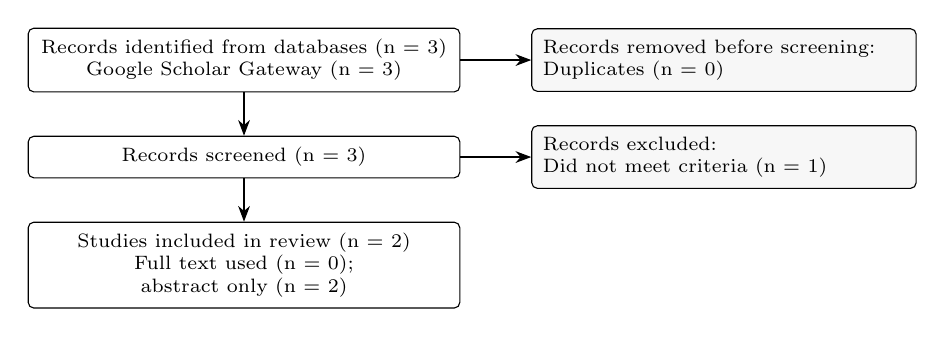
\begin{tikzpicture}[node distance=0.55cm and 0.9cm, font=\scriptsize,
  flowbox/.style={draw, rounded corners=2pt, align=center, text width=5.2cm, inner sep=4pt, fill=white},
  sidebox/.style={draw, rounded corners=2pt, align=left, text width=4.6cm, inner sep=4pt, fill=black!3},
  arrow/.style={-{Stealth[length=2mm]}}]
\node[flowbox] (id) {Records identified from databases (n = 3)\\ Google Scholar Gateway (n = 3)};
\node[sidebox, right=of id] (removed) {Records removed before screening:\\ Duplicates (n = 0)};
\node[flowbox, below=of id] (screened) {Records screened (n = 3)};
\node[sidebox, right=of screened] (excluded) {Records excluded:\\ Did not meet criteria (n = 1)};
\node[flowbox, below=of screened] (included) {Studies included in review (n = 2)\\ Full text used (n = 0); abstract only (n = 2)};
\draw[arrow] (id) -- (screened);
\draw[arrow] (screened) -- (included);
\draw[arrow] (id) -- (removed);
\draw[arrow] (screened) -- (excluded);
\end{tikzpicture}

\caption{PRISMA 2020 flow diagram of this run}
\end{figure}
\vspace{6pt}
\begin{figure}[H]
\centering
\begin{minipage}{0.32\textwidth}
\centering
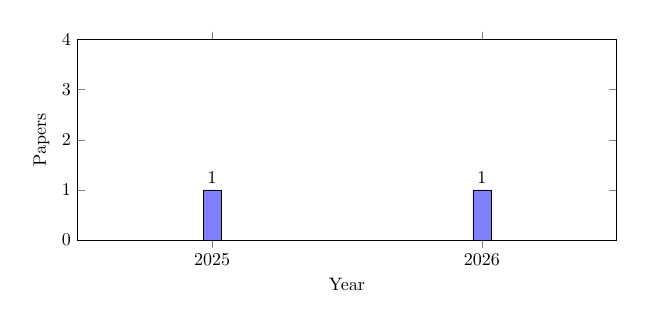
\begin{tikzpicture}[scale=0.65]
\begin{axis}[ybar, xtick={1,2}, xticklabels={2025,2026}, xmin=0.5, xmax=2.5, ymin=0, ymax=4, ylabel={Papers}, xlabel={Year}, nodes near coords, width=\textwidth, height=5.5cm, bar width=10pt]
\addplot[fill=blue!50] coordinates {(1,1) (2,1)};
\end{axis}
\end{tikzpicture}
\caption{Papers per Year}
\end{minipage}\hfill
\begin{minipage}{0.32\textwidth}
\centering
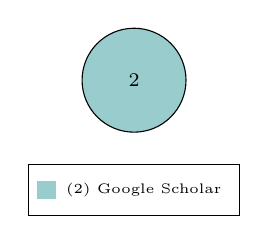
\begin{tikzpicture}[scale=0.55]
\draw[fill=teal!40] (0,0) circle (1.2cm); \node at (0,0) {\scriptsize 2};
\matrix [draw,below,matrix of nodes,font=\tiny,at={(current bounding box.south)},yshift=-0.4cm] {
\node[fill=teal!40,label=right:(2) Google Scholar] {}; & \\
};
\end{tikzpicture}
\caption{Platform Distribution}
\end{minipage}\hfill
\begin{minipage}{0.32\textwidth}
\centering
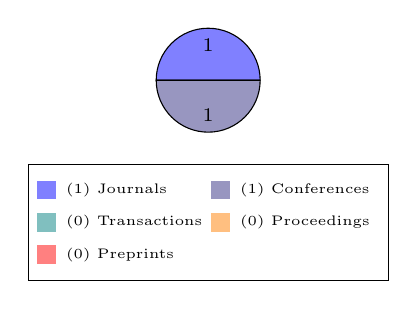
\begin{tikzpicture}[scale=0.55]
\draw[fill=blue!50] (0,0) -- (0:1.2cm) arc (0:180:1.2cm) -- cycle; \node at (90:0.8cm) {\scriptsize 1};
\draw[fill=customIndigo!50] (0,0) -- (180:1.2cm) arc (180:360:1.2cm) -- cycle; \node at (270:0.8cm) {\scriptsize 1};
\matrix [draw,below,matrix of nodes,font=\tiny,at={(current bounding box.south)},yshift=-0.4cm] {
\node[fill=blue!50,label=right:(1) Journals] {}; & \node[fill=customIndigo!50,label=right:(1) Conferences] {}; \\
\node[fill=teal!50,label=right:(0) Transactions] {}; & \node[fill=orange!50,label=right:(0) Proceedings] {}; \\
\node[fill=red!50,label=right:(0) Preprints] {}; & \\
};
\end{tikzpicture}
\caption{Venue Share}
\end{minipage}
\end{figure}
\vspace{10pt}
\small
\begin{tabularx}{\textwidth}{>{\hsize=0.6\hsize}X >{\hsize=1.2\hsize}X >{\hsize=1.0\hsize}X >{\hsize=0.5\hsize}X >{\hsize=1.7\hsize}X}
\multicolumn{5}{l}{\textbf{Table 3.1: Systematic Synthesis Extraction Registry}} \\\\
\toprule
\textbf{Paper Name} & \textbf{Executive Summary} & \textbf{Inclusion Rationale} & \textbf{Category} & \textbf{Citation (APA 7th)} \\
\midrule
Agent loops for safe orchestration & An agent paper & About agent architecture & Scholar & Doe, J. (2025). Agent loops for safe orchestration. \textit{Future Internet}. https://doi.org/10.3390/fi1234567 \\ \hline
Agent governance layers & An agent paper & About agent architecture & Scholar & Lee, K. (2026). Agent governance layers. In \textit{Proceedings of the Conference on Agents} \\ \hline
\end{tabularx}
\vspace{4pt}\noindent\small 
\textbf{Table Overview:} The extraction logs archived inside Table 3.1 summarize the qualitative characteristics of each selected paper.
\vspace{10pt}
\begin{tabularx}{\textwidth}{>{\hsize=0.25\hsize}X >{\hsize=0.8\hsize}X >{\hsize=1.1\hsize}X >{\hsize=0.9\hsize}X >{\hsize=1.95\hsize}X}
\multicolumn{5}{l}{\textbf{Table 3.2: Extracted Study Data}} \\
\toprule
\textbf{Ref.} & \textbf{Study type} & \textbf{Method} & \textbf{Sample} & \textbf{Key findings} \\
\midrule
{[}1{]} & design science artefact with evaluation & Supervisor checks & not reported & (1) Loops recover from faults \\ \hline
{[}2{]} & design science artefact with evaluation & Supervisor checks$^{\dagger}$ & not reported & (1) Loops recover from faults$^{\dagger}$ \\ \hline
\end{tabularx}
\vspace{2pt}\noindent\scriptsize $^{\dagger}$ The supporting quote given by the model was not found in the paper's text; treat the value with caution. Evidence: full text or abstract, see extraction.json.\normalsize
\vspace{10pt}
\begin{tabularx}{\textwidth}{>{\hsize=0.4\hsize}X >{\hsize=1.6\hsize}X c c c c c c}
\multicolumn{8}{l}{\textbf{Table 3.3: Quality Appraisal (MMAT 2018; Yes / No / ? = can't tell; Met = questions answered yes, not an overall score)}} \\
\toprule
\textbf{Ref.} & \textbf{Category} & \textbf{1} & \textbf{2} & \textbf{3} & \textbf{4} & \textbf{5} & \textbf{Met} \\
\midrule
{[}1{]} & quantitative descriptive & Yes & ? & ? & ? & ? & 1/5 \\
{[}2{]} & quantitative descriptive & ? & ? & ? & ? & ? & 0/5 \\
\bottomrule
\end{tabularx}
\vspace{10pt}
\vspace{10pt}
\begin{multicols}{2}
\section{Results \& Synthesis}
The findings of the 2 included studies were synthesised thematically. 2 studies yielded 2 codes, grouped into 1 theme: Recovery and oversight (2 studies). Each theme is reported in its own subsection below, and the evidence map shows which studies contribute to which theme
\subsection{Recovery and oversight}
Agent loops recover from faults through supervisor checks [1], while governance layers audit agent actions [2]
\par\smallskip\noindent\textit{The synthesis and discussion cite 2 of the 2 included studies}
\end{multicols}
\vspace{6pt}
\begin{tabularx}{\textwidth}{>{\hsize=0.9\hsize}X >{\hsize=1.4\hsize}X >{\hsize=0.7\hsize}X}
\multicolumn{3}{l}{\textbf{Table 4.1: Evidence Map of the Thematic Synthesis}} \\
\toprule
\textbf{Theme} & \textbf{Description} & \textbf{Studies} \\
\midrule
Recovery and oversight & How agent loops recover and are overseen & {[}1{]}, {[}2{]} \\ \hline
\end{tabularx}
\vspace{2pt}\noindent\scriptsize Second, independent coding: Cohen's kappa = 1.00 over 2 study-theme decisions\normalsize
\vspace{10pt}
\begin{multicols}{2}
\section{Discussion}
Recovery and audits complement each other [1, 2]
\subsection{Automated Citation Check}
An automated check compared the part of each cited sentence attributed to a paper with the text of that paper. Of 5 citations checked, 5 were judged supported, 0 partially supported, 0 not supported, and 0 could not be verified. Every verdict, with the quoted evidence, is listed in citation-audit.json; these are model judgements and should be spot-checked by a human reviewer
\section{Administrative Declarations}
\subsection{Support \& Funding}
No funding statement has been declared for this review. The funding and support text can be set in the Report:SupportStatement configuration value
\subsection{Registration and Protocol}
The review was not registered. Its protocol (search query, objective, eligibility criteria, sources, limits and screening set-up) was written to protocol.md on DATE (UTC) before any search was run, with SHA-256 fingerprint FINGERPRINT...; the extra search strings are appended to it as a dated amendment. The file is part of the run archive
\subsection{Open Science Code Availability}
The code of the tool (version VERSION) is openly available at https://github.com/lauPhilip/au-btech-literature-review-agent. The run archive contains the protocol, the raw source responses, the screening ledger, the extraction and appraisal data, the thematic codebook, every model call's fingerprint and a manifest.json with the SHA-256 fingerprint of every file. Journal quartiles are taken from the SCImago Journal Rank (SJR) data (https://www.scimagojr.com).
\end{multicols}
\clearpage
\begin{thebibliography}{99}
\bibitem{ref1} Doe, J. (2025). Agent loops for safe orchestration. \textit{Future Internet}. https://doi.org/10.3390/fi1234567
\bibitem{ref2} Lee, K. (2026). Agent governance layers. In \textit{Proceedings of the Conference on Agents}
\end{thebibliography}
\end{document}
